\documentclass[conference]{IEEEtran}
%\IEEEoverridecommandlockouts
% The preceding line is only needed to identify funding in the first footnote. If that is unneeded, please comment it out.
%\usepackage{cite}
\usepackage{amsmath,amssymb,amsfonts}
\usepackage{algorithmic}
\usepackage{graphicx}
\usepackage{textcomp}
\def\BibTeX{{\rm B\kern-.05em{\sc i\kern-.025em b}\kern-.08em
    T\kern-.1667em\lower.7ex\hbox{E}\kern-.125emX}}
\usepackage{mathtools}

\usepackage[backend=biber]{biblatex}
\addbibresource{references.bib}

\DeclareMathOperator*{\argmin}{argmin}
\DeclareMathOperator{\E}{\mathbb{E}}
\newcommand{\norm}[1]{\left\lVert#1\right\rVert}

\renewcommand*{\bibfont}{\footnotesize}

\begin{document}

\title{Optimal Control of Hybrid Energy Storages in Electric Vehicles}

\author{\IEEEauthorblockN{Alok Deshpande}
\IEEEauthorblockA{University of Toronto - Energy Systems}
}

%\newenvironment{psmallmatrix}
%  {\left[\begin{smallmatrix}}
%  {\end{smallmatrix}\right]}

\maketitle

%\begin{abstract}
%This document is a model and instructions for \LaTeX.
%This and the IEEEtran.cls file define the components of your paper [title, text, heads, etc.]. *CRITICAL: Do Not Use Symbols, Special Characters, Footnotes, 
%or Math in Paper Title or Abstract.
%\end{abstract}

\section{Introduction}
Battery life is a factor that is critical for electric vehicle (EV) operation. An aging battery experiences a drop in energy capacity \cite{shi2017optimal}, which reduces the maximum distance that can be travelled on a single charging. One promising way to prolong battery life is to use a hybrid energy storage system, composed of a combination of a battery and a secondary energy storage in parallel \cite{thounthong2009energy}, such as a supercapacitor \cite{bambang2014energy}\cite{thounthong2009energy}\cite{7939849}. 

Dynamic programming (DP) has previously been been applied in this context to determine an optimal sequence of controls -- that is to say, energy discharges from the battery and supercapacitor -- that satisfies a sequence of energy demands. \cite{su2013modeling} has employed DP with a black-box model of a single battery; we extend this to the two-storage case. Moreover, \cite{8330176} and \cite{8315074} have both solved the problem under the assumption of an infinite horizon, and we do so similarly.

However, our approach differs from these papers as we attempt to resolve the curse of dimensionality in the DP. We first reformulate the infinite horizon DP as a linear program (see, e.g., \cite{Bertsekas:2007:DPO:1396348}). We then construct an approximation using the technique given in \cite{deFarias:2003:LPA:970869.970918}. Finally, we generate basis functions for the approximation using the methods of \cite{Bellman:1957} and \cite{Bellman1962}. %\cite[pp. 323--324]{Bellman1962}.

We begin by modelling the problem in Section II and solving the exact equivalent problem in Section III. In Section IV, we explain how the basis functions are generated to approximate the solution to the exact LP, and hence we solve the approximate LP. Finally, in Section V, we show numerical results for the vehicle application and draw conclusions on the optimal response to various demand patterns. 

\section{Model}
In this section, we model the two storage device optimization problem. Let $E_{h}(t)$ and $D_{h}(t)$ denote the energy stored in and energy discharged from device $h$ at time instant $t$. Here $h=1$ refers to the battery and $h=2$ refers to the supercapacitor. Let $L(t)$ be the energy demand imposed on the system, and $C_{2}(t)$ be the energy input to the supercapacitor by charging. We define the state to be $x(t):=(E_{1}(t),E_{2}(t),L(t))$ and the control to be $u(t):=(D_{1}(t),D_{2}(t))$. Note that $C_{2}(t)$ is not part of the control because it is a dependent variable through the energy supply-demand balance, as explained below.

The state equation for the battery without regenerative braking is \begin{math}E_{1}(t+1)=\beta_{1}E_{1}(t)-\frac{1}{\alpha_{1}^{D}}D_{1}(t)\end{math}. Likewise, the state equation for the supercapacitor is \begin{math}E_{2}(t+1)=\beta_{2}E_{2}(t)+\alpha_{2}^{C}C_{2}(t)-\frac{1}{\alpha_{2}^{D}}D_{2}(t)\end{math}. Here, $\alpha^{C}_{h}$ and $\alpha^{D}_{h}$ respectively denote the charging and discharging efficiencies of device $h$, and $\beta_{h}$ is the leakage for device $h$.% The dynamics given by $f_{1}(\cdot)$ and $f_{2}(\cdot)$ can then be more generally represented by the function $f(x(t),u(t),w(t))$.

In this model, the energy in storage device $h$ is bounded in the range $E_{h}^{min}\leq E_{h}(t)\leq E_{h}^{max}$ where $E_{h}^{max}$ is the upper bound and $E_{h}^{min}$ is the lower bound, normally equal to zero. The charging and discharging are constrained to the ranges $0\leq C_{h}(t)\leq C_{h}^{max}$ and $0\leq D_{h}(t)\leq D_{h}^{max}$. The energy supply-demand balance imposes the following constraint: $D_{1}(t) + D_{2}(t) - C_{2}(t) = L(t)$.


There are two relevant costs in this model. The first is the loss of energy due to transfers between the devices, $(1-\alpha_{1}^{D})D_{1}(t)+(1-\alpha_{2}^{C})C_{2}(t)+(1-\alpha_{2}^{D})D_{2}(t)$. The other cost is that for the discharge rate for the battery, simply given by $K(D_{1}(t))^{2}$. Here $K$ is a weighting for this cost relative to the cost of energy loss. This cost penalizes larger excursions \cite{bambang2014energy}, which cause greater battery degradation.

The sum of these objective functions is convex non-negative. Hence, the following optimization problem -- whose objective is this sum -- has a unique solution:

\begin{multline} \label{eq:initCostFnc}
    \min_{D_{1},D_{2},C_{2}} \sum_{t=0}^{T-1}
	(1-\alpha_{1}^{D})D_{1}(t)+
	(1-\alpha_{2}^{C})C_{2}(t)+\\
	(1-\alpha_{2}^{D})D_{2}(t)+
	K\left[D_{1}(t)\right]^{2}
\end{multline}
subject to
\begin{displaymath}E_{h}^{min}\leq E_{h}(t)\leq E_{h}^{max}\end{displaymath}
\begin{displaymath}0\leq C_{2}(t)\leq C_{2}^{max}\end{displaymath}
\begin{displaymath}0\leq D_{h}(t)\leq D_{h}^{max}\end{displaymath}
\begin{displaymath}\left[D_{1}(t)\right] + \left[D_{2}(t) - C_{2}(t)\right] = L(t)\end{displaymath}
\begin{displaymath}E_{1}(t+1)=\beta_{1}E_{1}(t)-\frac{1}{\alpha_{1}^{D}}D_{1}(t)\end{displaymath}
\begin{displaymath}E_{2}(t+1)=\beta_{2}E_{2}(t)+\alpha_{2}^{C}C_{2}(t)-\frac{1}{\alpha_{2}^{D}}D_{2}(t)\end{displaymath} Note that the energy balance equality constraint can be immediately substituted into the objective and the charging inequality constraints, which reduces the decision vector to $u:=(D_{1},D_{2})$. %(More correctly, the minimization is done with respect to a vector $\textbf{D}$, whose components are $D(t)$ at $t=0,...,T-1$.  However, for the sake of clarity, we omit this formality.)

%Critically, this paper chooses to take the expectation after the minimization. This is done so that the net energy discharged (control, $D$) exactly matches the demand, $L$, at all times and not its expected value, ensuring supply-demand balance.

The optimal value function \eqref{eq:initCostFnc} may be expressed in the general form:
\begin{equation} \label{eq:FHDP}
	J^{*}(x(t))=\min \Biggl\{\mathop{\E}_{w}\left[\sum_{t=0}^{T-1}g(x(t),u(t),w(t))\right]\Biggr\}\end{equation}
where $g(\cdot)$ is the stage cost. The value function can then be re-written as a dynamic program:
\begin{displaymath}
J_{t}(x(t))=\min_{u(t)} g(x(t),u(t)) + \mathop{\E}_{w(t)} \{J_{t+1}(f(x(t),u(t),w(t)))\}
\end{displaymath}
starting from $J_{T}(x(T)):=0$. This is subject to the same constraints as \eqref{eq:initCostFnc}, which can be expressed as the set:
\begin{multline}
    \Omega = \left\{(E_{1},E_{2},L,D_{1},D_{2})\mid 
                E_{h}^{min}\leq E_{h}\leq E_{h}^{max}\\
                0\leq C_{2}(t)\leq C_{2}^{max}\\
                0\leq D_{h}(t)\leq D_{h}^{max}\\
                E_{1}(t+1)=\beta_{1}E_{1}(t)-\frac{1}{\alpha_{1}^{D}}D_{1}(t)\\
                E_{2}(t+1)=\beta_{2}E_{2}(t)+\left(\alpha_{2}^{C}C_{2}(t)-\frac{1}{\alpha_{2}^{D}}D_{2}(t)\right)
             \right\}
\end{multline} where $C_{2}=D_{1}(t)+D_{2}(t)-L(t)$, using the energy balance constraint.

In this model, $L(t)$ is a random quantity which is observed at time $t$ before the control $u(t)$ is applied because the controller must have full knowledge of the demand before providing the control to satisfy it. It evolves according to $L(t+1)=w(t)$, where $w(t)$ is a bounded random variable. Note that $w(t)$ depends on the energy in the subsequent state, $E(t+1):=(E_{1}(t+1),E_{2}(t+1))$. This is because the demand at any iteration cannot exceed the total current energy at that iteration. %$L(t+1)=0L(t)+w(t)$ which follows an unknown distribution and which represents a perturbation after the control is applied. %We have taken $L(t)$ to be part of the state. Doing so allows us to generate an optimal policy that a function of the load at time $t$, in addition to arbitrary energy state. (This choice of state makes the later LP formulation of this problem different from others reviewed in literature.)

We model the demand to further exhibit the Markov property. Firstly we define three sets: $W$ as the set of random perturbations, indexed by $k\in\{1,...,M\}$; $X$ as the set of states, indexed by $i\in\{1,...,NM\}$; and $U$ as the set of controls, indexed by $p\in\{1,...,P\}$. Here, $N$ is the cardinality of the set of vectors $(E_{1},E_{2})$. Furthermore, let $g(x_{i},u_{p})$ be the stage cost, and let $p_{i,j}(u_{p})$ be the probability of moving from $x_{i}\in X$ to $x_{j}\in X$ by applying control $u_{p}\in U$. Note that the subscripts are indices for vectors in the sets.

In terms of the above quantities, the probability $p_{i,j}(u_{p})$ is then: 
\begin{displaymath}
p_{i,j}(u_{p})= P(x_{j}| x_{i},u_{p})
\end{displaymath} For this probability to be non-zero, the next state $x_{j}$ must be a state $x_{i'}:=f(x_{i},u_{p},w_{k})$ that is accessible from the current state. In this case:
\begin{align*} 
p_{i,j}(u_{p})&= P(x_{i'}| x_{i},u_{p})\\ 
&= P(f(x_{i},u_{p},w_{k})| x_{i},u_{p})
\end{align*} The only random variable in the above expression is $w_{k}\in W$, so we may express this instead as a probability of $w_{k}$:
\begin{align*} 
p_{i,j}(u_{p})&= P(w_{k} | x_{i},u_{p})
\end{align*} This finally shows that the random demand in the subsequent state does not depend on the demand in states before the current, $x_{i}$. 

%-- i.e. we assume that vehicle will not be completely depleted of fuel. However, the subsequent energy depends on the current energy through $f(\cdot)$, so in a manner respecting causality, the above expectation is more correctly conditioned on $x(t)$ and $u(t)$. While this conditioning is not shown, we do assume that the process generating $w(t)$ is Markovian.

%It is common knowledge that a finite number of iterations is sufficient to allow $J_{t}[x(t)]$ to reach a steady-state value of $J^{*}(x)$ within a tolerance $\epsilon$. The method of solving these multiple iterations is called discounted value iteration with bounded cost per stage. In Section V, we explain how we set this tolerance compared to that in the LP formulation. LP is now presented below.

%This DP program can be analyzed to determine its computational complexity. Firstly, with regards to the size of the problem, two matrices must hold data: the optimal cost, and the optimal control. By inspecting (6), it is clear that both the cost and control are functions of the state $(x,w)$, and so must have a size of $N\times M$. However, the previous costs must also be retained to determine that the costs are converging, so the required size is actually twice that (two matrices).

%The theoretical runtime can also be analyzed. Knowing that each iteration of DP involves nothing more than exhaustive searching (cost evaluation), and that $g(\cdot)$ is a function of the triplet $(x,u,w)$, the number of combinations to evaluate must be $NMP$. Over $k$ iterations, this is then $NMPk$ evaluations. According to theory \cite{Bertsekas:2007:DPO:1396348}, $k$ is related to the logarithm of the error tolerance on the constraints, and so it is also possible to estimate runtime in theory. However, this paper chooses to test the number of iterations from numerical examples, as detailed in Section 8.

%These computational characteristics for the DP will be compared to those of the LP, which is now presented below.


\section{Infinite Horizon Approximation}
%\subsection{Infinite Horizon DP}
The length of each time period is very small relative to the total driving time. For example, each period might represent a second. If the total driving time is an hour, this means 3600 periods. This motivates the use of an infinite horizon approximation.

%The above problem can be solved for $T$ control periods. However, for the very large number of periods required in this application, the total value $J$ will approach infinity, since each stage cost is non-negative. Thus, it is necessary to discount future costs by a factor $0<\alpha<1$.

%With this modification, over multiple iterations the value function $J_{t}[x(t)]$ approaches the steady-state function $J(x)$. When a greedy policy is selected at each iteration, this function $J(x)$ is also optimal ($J^{*}(x)$). Hence, 
With a modification to \eqref{eq:FHDP}, the infinite horizon problem is:
\begin{multline} \label{eq:DP}
J^{*}(x)= \min\Biggl\{\mathop{\E}_{w}\left[\sum_{t=0}^{\infty}\alpha^{t}g(x(t),u(t),w(t))\right]\Biggr\}
\end{multline} subject to $(x(t),u(t))\in\Omega \hspace{0.1cm}\forall t$, where $(x(t),u(t))$ is a vector comprised of both a state-control pair at time $t$. Here $\alpha$ is a real-valued discount factor such that $0<\alpha<1$. Using this approximation, in the following sections we formulate the LP that the equivalent to this DP and solve the dual LP to obtain the optimal policy.

%When subject to the same constraints as \eqref{eq:initCostFnc}, this optimization problem is termed the infinite horizon DP formulation of optimal control for this paper. However, because we only use the infinite horizon approach for this application, henceforth we will simply use \textit{DP} to refer to this infinite horizon DP.

\subsection{Linear Programming Formulation}
%Given that the value $J_{t}[x(t)]$ approaches an upper bound of $J^{*}(x)$, as shown in \cite{Bertsekas:2007:DPO:1396348}, $J^{*}(x)$ can be calculated by solving an LP maximization problem. This LP has optimal \textit{solution} of $J^{*}(x)$, rather than its optimal value as in value iteration, so henceforth we use \textit{costs} of the LP to refer to the possible solutions and not values of the LP objective function.

In \cite{Bertsekas:2007:DPO:1396348}, Bertsekas presents an LP formulation of the infinite horizon DP where the state has no uncontrollable components (in this case, the demand) that are randomly generated. We rewrite this in a form where the uncontrollable component is part of the state.

To this end, let $\lambda(x_{i})$ be the cost associated with state $x_{i}$ such that $\boldsymbol{\lambda(x)}$ is a vector with the elements being costs in each state. Then, the LP is:

\begin{equation} \label{eq:prelimLP}
\min_{\lambda(x_{i}) \forall i} \sum_{i=1}^{NM} -\lambda(x_{i})
\end{equation}

subject to $\forall x_{i} \in X$: \begin{align*}
\lambda(x_{i})-\alpha\sum_{k=1}^{M}P(w_{k} | x_{i},u_{1})\lambda(f(x_{i},u_{1},w_{k})) &\leq g(x_{i},u_{1}) \\
&\vdots\\
\lambda(x_{i})-\alpha\sum_{k=1}^{M}P(w_{k} | x_{i},u_{P})\lambda(f(x_{i},u_{P},w_{k})) &\leq g(x_{i},u_{P})
\end{align*} This is the LP whose solution is the same as the optimal value of \eqref{eq:DP}. As a reminder, in the context of the hybrid storage problem, $x=(E_{1},E_{2},L)$ and $u=(D_{1},D_{2})$.

The problem can be expressed most succinctly in matrix form as:
\begin{equation} \label{eq:prelimLPmtx}
    \max_{\boldsymbol{\lambda_{p}}} \boldsymbol{1}^{T} \boldsymbol{\lambda_{p}}
    \hspace{1em}s.t.\hspace{1em}
    \boldsymbol{\lambda}-\alpha PF\boldsymbol{\lambda} \leq \boldsymbol{g}
\end{equation} Here, $\boldsymbol{\lambda} = [\boldsymbol{\lambda_{p}}\hdots \boldsymbol{\lambda_{p}}]^{T}$ is a vector containing P repeated vectors $\boldsymbol{\lambda_{p}}$. Each vector $\boldsymbol{\lambda_{p}}$ contains the current state costs, $\lambda(x_{i})$, as its components. Likewise, the vector $F\boldsymbol{\lambda}$ contains P repeated vectors each containing the costs for next states $x_{j}$, which are $\lambda(x_{j})$. And finally, vector $\boldsymbol{g}$ contains the stage cost for each state-control pair. 

In addition to this, $P$ is a transition probability matrix containing the conditional probabilities $p_{i,j}$. For the subset of its rows associated with the $p^{th}$ control -- i.e. the $p^{th}$ set of inequalities in \eqref{eq:prelimLPmtx} -- these probabilities are $p_{i,j}(u_{p})$. Hence, based on the prior definition of these elements $p_{i,j}(u_{p})$, one may note that its structure is:

\begin{displaymath}
p_{i,j}(u_{p}):=
\left\{
\begin{array}{l}
P(w_{k}|x_{i},u_{p}) \hspace{0.2cm} \text{if} \hspace{0.2cm} x_{j}=f(x_{i},u_{p},w_{k})\\
0 \hspace{1.8cm} \text{otherwise}
\end{array}
\right.
\end{displaymath}

%Firstly, one can consider just the subset of costs associated with the $p^{th}$ control. This is done because each of the sets of linear inequalities in \eqref{eq:prelimLP} -- i.e. all of the inequalities for fixed $p$ -- is of the same form, so the full matrix formulation will consist just of the concatenation of the individual matrix equations. For the $p^{th}$ control, the $p^{th}$ expression on the left in the set of linear inequalities of \eqref{eq:prelimLP} can be expressed in the form:

%\begin{gather}\label{eq:mtxLPineq}
%\begin{psmallmatrix}
%& \lambda_{1}\\
%& \vdots\\
%& \\
%& \lambda_{NM}
%\end{psmallmatrix}
%-
%\alpha PF\begin{psmallmatrix}
%& \lambda_{1}\\
%& \vdots\\
%& \\
%& \lambda_{NM}
%\end{psmallmatrix}\end{gather}


The optimization in \eqref{eq:prelimLPmtx} cannot yet be solved without knowing the form of $F$. One may determine $F$ by relating the next state costs to the current state costs. Since every triplet $(x_{i},u_{p},w_{k})$ leads to a next state $x_{i'}=f(x_{i},u_{p},w_{k})$ that lies in the same set as the current state (set $X$), this implies that $F$ is a permutation mapping defined as:

\begin{displaymath}
F_{j,i}:=
\left\{
\begin{array}{l}
1\hspace{0.2cm} \text{if} \hspace{0.2cm}x_{j}=x_{i}\\
0\hspace{0.2cm} \text{otherwise}
\end{array}
\right.
\end{displaymath} Unlike previously, in this case $j$ denotes the row and $i$ denotes the column.

Having determined the forms of $P$ and $F$, the LP in \eqref{eq:prelimLPmtx}, which is:
\begin{equation} \label{eq:LPfinal}
    \max_{\boldsymbol{\lambda_{p}}} \boldsymbol{1}^{T} \boldsymbol{\lambda_{p}}
    \hspace{1em}s.t.\hspace{1em}
    (I-\alpha PF)\boldsymbol{\lambda} \leq \boldsymbol{g}
\end{equation} can be solved. This is the final form of the LP exactly equivalent to the DP. 

\subsection{Dual LP}
This exact LP does not allow for directly determining the optimal policy upon convergence. Hence, it is necessary to reformulate it as the dual LP described in \cite{4220813}.

The dual LP can be expressed as:
\begin{equation}
    \max_{\boldsymbol{d}} -\boldsymbol{g}^{T} \boldsymbol{d}
    \hspace{1em}s.t.\hspace{1em}(I-\alpha PF)^{T}\boldsymbol{d} - \boldsymbol{1} = \boldsymbol{0}\hspace{1em}\boldsymbol{d} \geq \boldsymbol{0}
\end{equation}
where $\boldsymbol{d}$ is a vector of Lagrange multipliers for each state-control pair. Then, define $\pi$ to be the policy matrix, containing in its entries each probability of an action $u$ in a state $x$. At last, we determine the optimal policy, $\pi^{*}$, as follows, according to \cite{4220813}:

\begin{equation}
\pi^{*}(x,u)=\frac{d^{*}(x,u)}{\sum_{\forall u \in U}d^{*}(x,u)}
\end{equation} Here $\boldsymbol{d^{*}}$ is the optimal solution to the dual LP.

Note that when the solution is searched on the vertices of the constraints, the matrix $\pi$ is purely deterministic \cite{MDPs}. This is to say it only contains binary entries, so the most optimal elements (control values at each state) are chosen with probability 1. Because a random control policy should be avoided, this means that the solution algorithm should only search on the vertices. For this reason, the simplex method is chosen in numerical solutions.

In practice, we modify the above program by removing infeasible states. In this application, these are states where the inequality constraints in \eqref{eq:initCostFnc} are violated. Notably, removing states reduces the number of decision variables, and so can make solving the LP a less computationally complex alternative to the DP. The reader may refer to other sources for a detailed comparison of the computational complexity of the two programs.

\section{Approximate Solution of DP}

The major issue which prevents us from solving this DP exactly is that the size of the state space grows exponentially in the number of decision variables \cite{deFarias:2003:LPA:970869.970918}. To resolve the curse of dimensionality, we approximate the value function by a parametric architecture. %, where $r$ is a parameter vector of weights. By limiting the 

A common choice of architecture is linear, which has the form $\lambda\approx \Phi r$ where $\Phi$ is termed the design matrix and $r$ is a vector of weights. The $q^{th}$ column vector of $\Phi$ is a basis function denoted by $\phi_{q}$. The choice of basis functions depends on the problem, and may significantly impact the normalized approximation error for this architecture, which we define as $\norm{J^{*}-\Phi r}\div\norm{J^{*}}$. In this section, we develop a method to generate basis functions for the two-storage problem that empirically allow for low approximation error given a constant number of decision variables in vector $r$.

As explained in \cite{deFarias:2003:LPA:970869.970918}, the choice of state-relevance weightings, $c$, greatly impacts the approximation error for each state. Upon weighting the approximate optimal value in each state for the DP solution, the objective of this program is to maximize $c^{T}\Phi r$. However, \cite{deFarias:2003:LPA:970869.970918}, \cite{PatrascuReluEugen2004} and many others note that there is no known procedure for determining the optimal state-relevance weights. Hence, we choose equal weightings for all states, such that the approximate LP for this application is:
\begin{equation} \label{eq:ApproxLP}
    \max_{\boldsymbol{r}} \boldsymbol{1}^{T} \Phi r
    \hspace{1em}s.t.\hspace{1em}
    (I-\alpha PF)\Phi r \leq \boldsymbol{g}
\end{equation}

We now describe methods to generate the basis functions. We determined from literature review and testing with numerical examples that the three methods of monomials, randomly generated bases, and state aggregation and are effective for this application. Hence, in Subsections IV-A -- IV-C, we describe how we apply them respectively to design $\Phi$ in this application. Subsequently, in Section IV-D, we combine the three methods and explain how this heuristic method permits a trade-off between the number of basis functions -- and hence the number of decision variables -- and approximation error. Data for the approximation error using this method will be shown for the numerical examples in Section VI.

\subsection{Monomials}
    Assuming the value function is an analytic function of the state, one method of designing the matrix $\Phi$ is to choose the bases to be monomial functions of the state index for each state \cite{bertsekas1995dynamic}\cite{478953}. Let $R$ be the highest order of monomial. This would mean that the matrix $\Phi$ has the form:
	
	\begin{displaymath}
        \Phi_{i,j}:=s(i)^{j-1}
    \end{displaymath}. Here $i$ is the state index, $j\in\{1,2...,R+1\}$ is the column index, and $s(i)$ is a function which maps the state index to the associated state. Again, a trade-off exists for increasing the value of $R$ between more decision variables and lower approximation error.
	
	%\begin{gather}
    %    \Phi
    %    =
    %    \begin{bmatrix}
    %    \bold{1} & \bold{i} & \bold{i^{2}} & \bold{i^{3}} & \hdots & \bold{i^{R}}\\
    %    & & \vdotswithin\\
    %    \end{bmatrix}
    %\end{gather} 

\subsection{Random Vectors}
    It is known that adding any linearly independent vector to an existing basis is guaranteed to decrease the approximation error. For that reason, we can sample randomly generated vectors until determining an additional vector that is linearly independent from the current basis, and subsequently add it to the basis. We can repeat this an arbitrary number of times to improve the approximation.


 \subsection{State Aggregation}
    
    One may consider the case where multiple states have sufficiently similar optimal values that it is possible to approximate each optimal value by a single value for all the states in that aggregation. We can also use this to reduce the number of decision variables down to the number of aggregations \cite{5717627}. Specifically, each state in the aggregation has an associated index, so the basis functions are many-to-one functions of the state index $i$.
    
    Appropriate state aggregations depend on the problem, since the optimal value function varies. By grouping state indices giving constant values of a function $b(i)$, we can determine the minimum number of aggregations to approximate the value function. Since each aggregation must have the same value of $J^{*}_{j}(i) = \phi_{j}(i)r_{j}$ this implies that the matrix $\Phi$ must have the form:
    
    \begin{displaymath}
        \Phi_{i,j}:=\left\{
            \begin{array}{l}
            1 \hspace{0.2cm} \text{if} \hspace{0.2cm} i\in H_{j}\\
            0 \hspace{0.2cm} \text{if} \hspace{0.2cm} i\not\in H_{j}
            \end{array}
            \right.
    \end{displaymath}where $H_{j}$ is the set $\{i|f_{j} = \phi_{j}(i)r_{j}\}=\{i|e_{j} = b(i)\}$. Here, $f_{j}$ and $e_{j}$ are, respectively, the approximate optimal value and the constant value of $b(i)$ associated with the $j^{th}$ aggregation (basis vector).
    
    Since each value of state index has an associated state, we can treat $b$ to be a function of the state instead. By observing a sampling of the optimal values from solving the DP exactly, we can then deduce a form for $b(E_{1},E_{2},L)$ such that the sets $H_{j}$ have more than one element. For example, we determine empirically that for this model the function $b(E_{1},E_{2},L)=L-E_{2}$ has approximately this property. However, because it is model dependent, it only applies for the linear state equations:
	\begin{displaymath}E_{1}(t+1)=\beta_{1}E_{1}(t)-\frac{1}{\alpha_{1}^{D}}D_{1}(t)\end{displaymath}
	\begin{displaymath}E_{2}(t+1)=\beta_{2}E_{2}(t)+\alpha_{2}^{C}[D_{1}(t)+D_{2}(t)-L(t)]-\frac{1}{\alpha_{2}^{D}}D_{2}(t)\end{displaymath}
	
	Let $n$ be the dimension of the space containing the value function, which for this model is four. The function $b(E_{1},E_{2},L)=L-E_{2}$ gives an approximation of the level sets of the value function over the state space because the level is approximately constant in affine subspaces of dimension $n-2$ that are tangent to the level sets. Since the state is discretized, there may be up to as many aggregations as there are these subspaces. When increasing the number of aggregations by adding more terms to $b(E_{1},E_{2},L)$, there is then a trade-off between more decision variables and lower approximation error. %combinations of the components of the state with terms in $b(E_{1},E_{2},L)$
	
	In order to generate a form for $b(E_{1},E_{2},L)$ that applies for another model with different linear state equations, we present a simple heuristic. It is known that one step of value iteration provides an approximation of the optimal value. Moreover, we are able to discretize the state with a much finer resolution without being affected by the curse of dimensionality. Hence, we are able to determine aggregations of states that have similar values based on this single iteration, which makes state aggregation more applicable to other models.
    

\subsection{Combination of Approximations}
    
    We could approximate the value function by monomial basis functions as just described. However, let us assume that its level sets can be approximated by the affine subspaces mentioned in Subsection IV-C such that the number of aggregations is fewer than the number of states. In this case, we can reduce the approximation error using $R'$ state aggregation basis vectors more than by an arbitrary selection of the same number of monomials basis vectors, where $R'<R$. We can then add $R''-R'$ monomial basis vectors to account for deviations in value that lead the assumption to be only partially correct. Finally, we add $R-R''$ linearly independent random basis vectors to improve the approximation. This will permit lower approximation error than the method in Section IV-A for the same number of basis vectors ($R$).
    
    %we empirically observe that when the state dynamics are linear, the weighting of the constant and linear monomials are much greater than those of the higher order terms up to monomials of order $R$. This suggests that approximating the affine component is more significant in reducing the approximation error.
    
    Hence, we propose our own heuristic of choosing the basis vectors for value function approximation: combining the methods of state aggregations and monomial bases. This can provide a full approximation of the value function. The associated design is:
    
    \begin{displaymath}
        \Phi_{i,j}:=\left\{
            \begin{array}{l}
            1 \hspace{0.2cm} \text{if} \hspace{0.2cm} i\in H_{j} \hspace{0.2cm} \text{and} \hspace{0.2cm} 1\leq j\leq R'\\
            0 \hspace{0.2cm} \text{if} \hspace{0.2cm} i\not\in H_{j} \hspace{0.2cm} \text{and} \hspace{0.2cm} 1\leq j\leq R'\\
            s(i)^{j-1-R'} \hspace{0.2cm} \text{if} \hspace{0.2cm} (R'+1)\leq j\leq R''\\
            \xi \hspace{1.6cm} \text{if} \hspace{0.2cm} (R''+1)\leq j\leq R
            \end{array}
            \right.
    \end{displaymath} Here $\xi$ is a Bernoulli random variable whose probability distribution is conditioned on the other basis vectors such that the randomly generated vector $\phi_{j}$ with $(R'+1)\leq j\leq R''$ is linearly independent of the other basis vectors.
    
    Based on empirical tests done in Section VI, this is the best approximation of the value function for the fewest number of vectors amongst those considered.







\section{Interpolation}
In general, the next state of the MDP need not belong to the set of discrete states, X. We call the occurrence when the state is not in X as the state $\textit{falling off the grid}$ of discretization. To determine the cost-to-go of a next state which is off the grid, we choose to interpolate the value function between states. This allows us to solve the MDP offline more accurately.

Let $\lambda(x_{j})$ be the value of a state $x_{j} \not\in X$, and $\lambda(x_{i'})$ be the value of the $i'^{th}$ state in $X$, $x_{i'}$. We denote this as $x_{i'}$ because $x_{j}=f(x_{i}, u, w)$ is a next state which falls off the grid and $x_{i'}$ neighbours $x_{j}$. 

We use multilinear interpolation, as defined in [1], for simplicity. This gives:
\begin{displaymath}
	\lambda(x_{j})=\sum_{i'}^{MN}q_{i',j}\lambda(x_{i'})
\end{displaymath} Here, $MN$ is the cardinality of $X$, and $q_{i',j}$ are weightings that depend on the manner of the interpolation. The weightings have the property $0\leq q_{i',j}\leq 1$

The expected cost to go to state $x_{j}$ from state $x_{i}$ is then:
\begin{displaymath}
    \mathop{\E}_{w}\{\lambda(f(x_{i},u,w))\}=\sum_{j}\sum_{i'}^{MN}p_{i,j}(u)q_{i',j}\lambda(x_{i'})
\end{displaymath} We use this to alter the constraint in \eqref{eq:prelimLP} to account for states off the grid, as given by the second constraint in \eqref{eq:interpLP}.

For this model, the state has only two components that can be off the grid ($E_{1}$ and $E_{2}$), since the demand is a discrete random variable that lies in the set $W$ by definition. Hence, we use bilinear interpolation for the weightings.

Let $a:=E_{1}$ and $b:=E_{2}$ be the two components. Furthermore, let $\bold{i'}=(l',m')$ replace $i'$ to refer to the indices of the two energy components in their respective sets individually. This is to say that $a_{l'}\in X_{1}\hspace{0.1cm}\forall\hspace{0.1cm}l'\in\{1,2,...\}$ and $b_{m'}\in X_{2}\hspace{0.1cm}\forall\hspace{0.1cm} m'\in\{1,2,...\}$, where $X_{1}$ and $X_{2}$ are sets of the battery and supercapacitor discrete energy levels respectively. %when (a,b,L)\in X \forall L \in W.
Then, the weightings for bilinear interpolation are:
\begin{displaymath}
    q_{\bold{i'},j}:=q_{l',m',j}=(1-\frac{a_{j}-a_{l'}}{a_{l'+1}-a_{l'}})(1-\frac{b_{j}-b_{m'}}{b_{m'+1}-b_{m'}})
\end{displaymath} Here, $a_{j}$ and $b_{j}$ are components of the state $x_{j}\not\in X$. They have the properties that $a_{l'}\leq a_{j}< a_{l'+1}$ and $b_{m'}\leq b_{j}< b_{m'+1}$. Furthermore, $q_{l',m',j}:=0\hspace{0.2cm}$ for states on the grid where these constraints are not satisfied.

%\begin{displaymath}
%q_{l',m',j}:=
%\left\{
%\begin{array}{l}
%(1-\frac{a_{j}-a_{l'}}{a_{l'+1}-a_{l'}})(1-\frac{b_{j}-b_{m'}}{b_{m'+1}-b_{m'}}) \hspace{0.2cm} \text{if} \hspace{0.2cm}a_{l'}\leq a_{j}<a_{l'+1} \text{and} b_{m'}\leq b_{j}< b_{m'+1}\\
%0\hspace{0.2cm} \text{otherwise}
%\end{array}
%\right.
%\end{displaymath}

With this interpolation, the full LP can be expressed as:

\begin{equation} \label{eq:interpLP}
\max_{\lambda(x_{i}) \forall i} \sum_{i=1}^{NM} \lambda(x_{i})
\end{equation} subject to, $\forall (x_{i}, u_{p}, w_{k})\in(\Psi_{1}\cap\Psi_{2})$:
\begin{displaymath}
    \lambda(x_{i})-\alpha\sum_{k=1}^{M}P(w_{k} | x_{i},u_{p})\lambda(f(x_{i},u_{p},w_{k})) \leq g(x_{i},u_{1})
\end{displaymath} where $\Psi_{1}=\{(x_{i}, u_{p}, w_{k})|f(x_{i}, u_{p}, w_{k})\in X\}$, $\Psi_{2}=\{(x_{i}, u_{p}, w_{k})|(x_{i}, u_{p})\in\Omega, w_{k}\in W\}$. It is also subject to, $\forall (x_{i}, u_{p}, w_{k})\in(\Psi_{1}^\complement\cap\Psi_{2})$:
\begin{displaymath}
    \lambda(x_{i})-\alpha\sum_{k=1}^{M}P(w_{k} | x_{i},u_{p})\sum_{i'}^{MN}q_{i',j}\lambda(x_{i'}) \leq g(x_{i},u_{p})
\end{displaymath}

As before, we can rewrite this in the condensed form:
\begin{equation}
    \max_{\boldsymbol{\lambda_{p}}} \boldsymbol{1}^{T} \boldsymbol{\lambda_{p}}
    \hspace{1em}s.t.\hspace{1em}
    (I-\alpha PF)\boldsymbol{\lambda} \leq \boldsymbol{g}
\end{equation} We modify the matrix F, however, to correspond with the above constraints. Let $l$ denote the row and $i$ the column of F. Then:
\begin{displaymath}
F_{l,i}:=
\left\{
\begin{array}{l}
1		   \hspace{1cm} \text{if} \hspace{0.2cm}x_{l}=x_{i}, \hspace{0.1cm}x_{l}\in X\\
q_{l',m',l}\hspace{0.2cm} \text{if} \hspace{0.2cm} a_{l'}\leq a_{l}< a_{l'+1}, b_{m'}\leq b_{l}< b_{m'+1}, x_{l}\notin X\\
0		   \hspace{1cm} \text{otherwise}
\end{array}
\right.
\end{displaymath} Here $x_{i}\in X$ and so can be expressed as $x_{i}:=(a_{l'},b_{m'},L)$ for any $L\in W$. Likewise, $x_{l}$ may not belong to X, and so can be expressed as $x_{l}:=(a_{l},b_{m},L)$ for any $L\in W$.

Finally, let $\lambda\approx \Phi r$, as before. Then, the approximate LP with interpolation is:
\begin{equation}
    \max_{\boldsymbol{r}} \boldsymbol{1}^{T} \Phi r
    \hspace{1em}s.t.\hspace{1em}
    (I-\alpha PF)\Phi r \leq \boldsymbol{g}
\end{equation}
where $F$ is defined as above. This is the LP we solve to determine the optimal policy offline.

Subsequently, we also interpolate the optimal controls when applying the optimal policy online. This allows us to approximate the minimum cost trajectory if the state falls off the grid as the MDP transitions between states. 

Let $u^{*}(x_{j})$ be the optimal control to apply in a state $x_{j} \notin X$. Specifically, define $x_{j}$ to have a demand component of $L_{0}$. Then, we also approximate $u^{*}(x_{j})$ using bilinear interpolation as:

\begin{equation}
    u^{*}(x_{j})=\sum_{l',m'}q_{l',m',j}u^{*}(a_{l'},b_{m'},L_{0})
\end{equation} where the state $(a_{l'},b_{m'},L_{0})\in X$ and $q_{l',m',j}$ is as defined above.
    
    
    

\section{Numerical Examples}
To test the optimal policy, we run it online with data based on the energy storage application. In this paper, the optimization problems were solved numerically in MATLAB for varying sizes of state space (cardinality $NM$) and $\epsilon$, with all other variables kept constant. Using discount $\alpha=0.99$, efficiency factors $\alpha_{C}=0.99$, $\alpha_{D}=0.9$, and $\beta=0.99$ based on \cite{su2013modeling}, and $K=2$, the problems were solved to determine the optimal policy offline. Then, demand sequences where the random load followed a uniform distribution were applied to determine how the battery and supercapacitor should behave under different conditions with the policy.

Having removed the infeasible states, the approximate LP was first solved offline. The optimal policy was then tested online with three broad cases of demand: 1) constant, 2) ramp (continuously increasing/decreasing), and 3) fluctuating. Each demand sequence was randomly generated following a uniform distribution, for simplicity. Importantly, no excess demands were permitted based on the state (total energy stored), such that the conditional probabilities could still change over time as the state evolved.

In the case of a constant or ramp demand, it was determined that the battery will tend to supply the majority of the energy. Figures \ref{fig:ConstDemand} and \ref{fig:RampDemand} illustrate these two cases for one set of initial conditions.
\begin{figure}[htbp]
\centerline{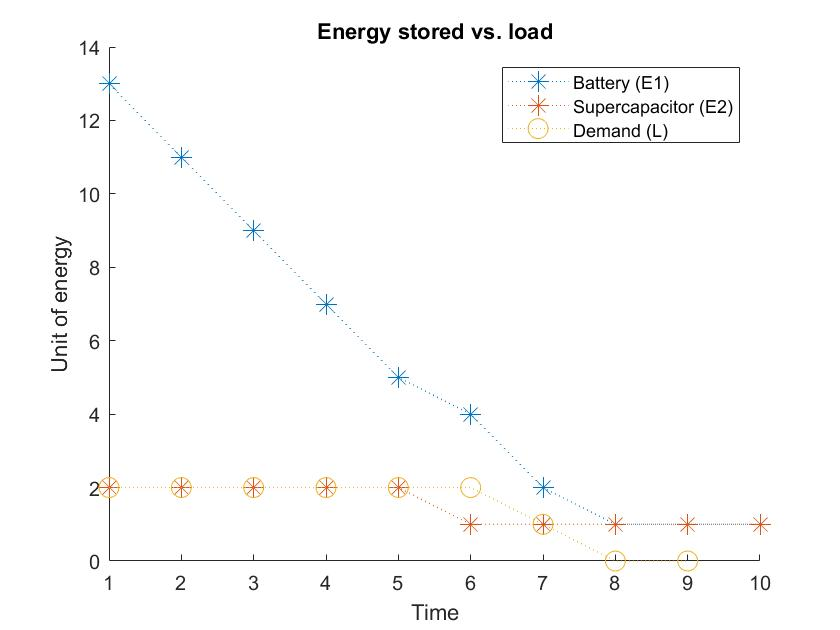
\includegraphics[scale=0.25]{EnergyStoredvsload_ConstantLoad(E1_max=13,E2_max=2).jpg}}
\caption{Testing optimal policy online with a constant demand sequence. Test size: N=$14\cdot3=42$, M=16.}
\label{fig:ConstDemand}
\end{figure}
\begin{figure}[htbp]
\centerline{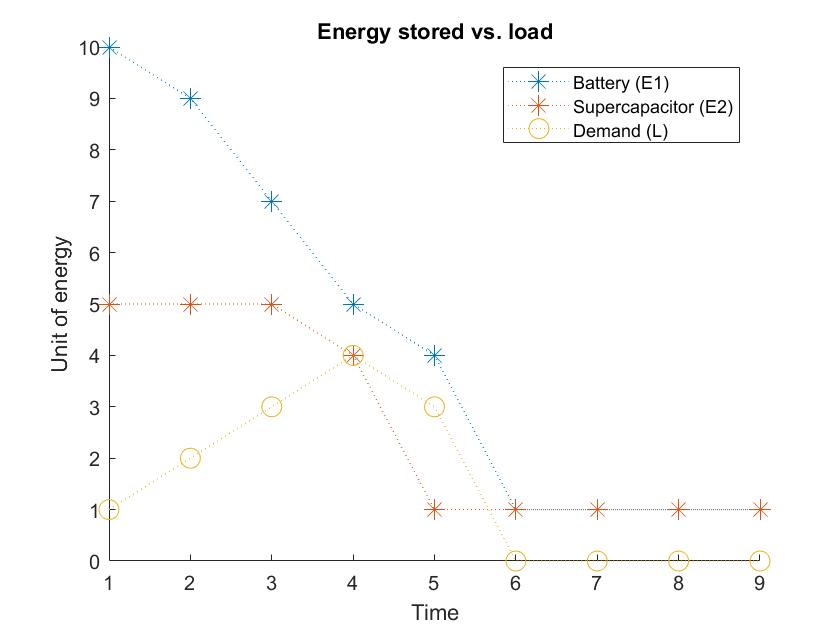
\includegraphics[scale=0.25]{EnergyStoredvsload_RampLoad(E1_max=10,E2_max=5).jpg}}
\caption{Testing optimal policy online with a ramp demand sequence. Test size: N=$11\cdot6=66$, M=16.}
\label{fig:RampDemand}
\end{figure} This result is expected because there is low cost for steady use of the battery (constant demand) or for limited cycling (ramp demand).

On the other hand, for fluctuating demand, the supercapacitor is used more, as illustrated in Figure \ref{fig:FluctuatingDemand}.
\begin{figure}[htbp]
\centerline{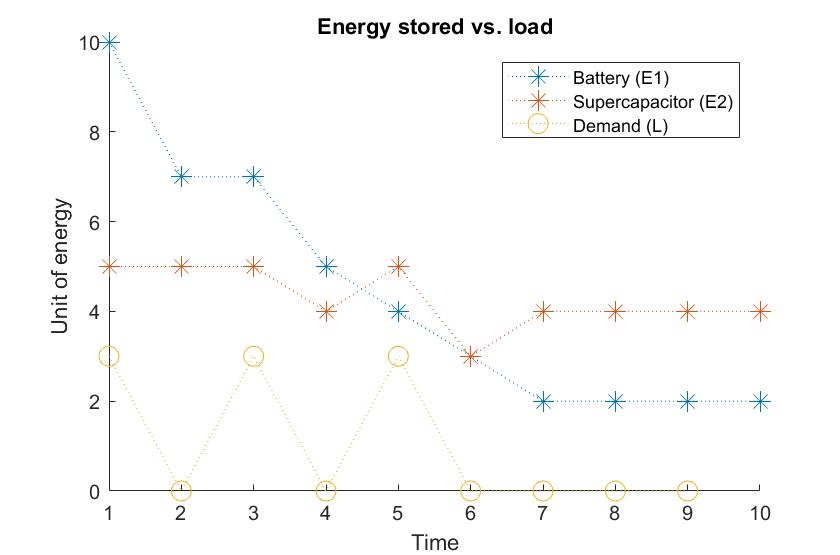
\includegraphics[scale=0.25]{EnergyStoredvsFluctuatingLoad(E1=10,E2=5).jpg}}
\caption{Testing optimal policy online with a fluctuating demand sequence. Test size: N=$11\cdot6=66$, M=16.}
\label{fig:FluctuatingDemand}
\end{figure} Clearly, the supercapacitor is now discharged at the start. However, this is still not as much use as expected. It was observed that by reducing the discharging efficiency of the battery, the supercapacitor is used more often (see Figure \ref{fig:FluctuatingDemand_LowBattEff}).
\begin{figure}[htbp]
\centerline{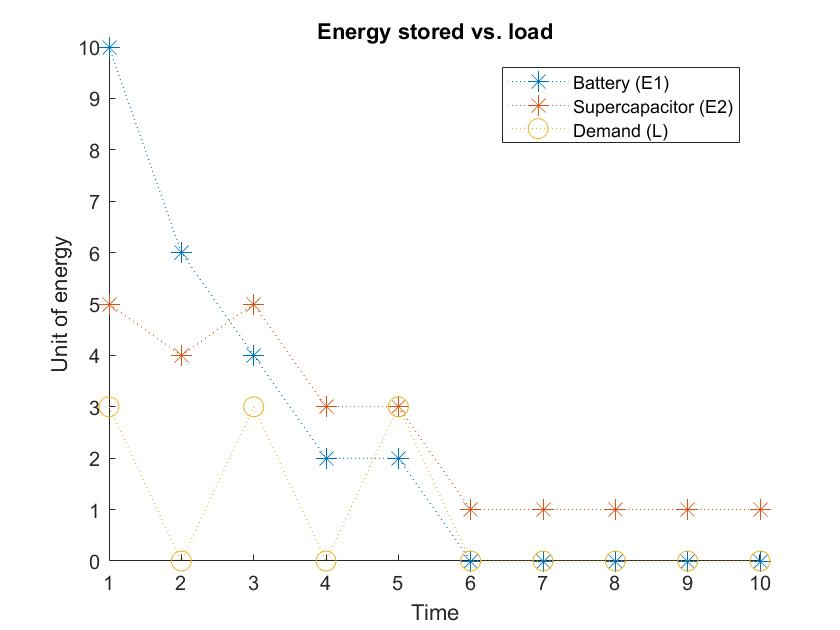
\includegraphics[scale=0.25]{EnergyStoredvsFluctuatingLoad_LowBattEff(E1=10,E2=5).jpg}}
\caption{Testing optimal policy online with a fluctuating demand sequence. Test size: N=$11\cdot6=66$, M=16. Lower battery efficiency (50\%).}
\label{fig:FluctuatingDemand_LowBattEff}
\end{figure} Hence, it is concluded that discharging the battery at the start of the sequence is still preferred because of the higher probability of large initial demands, unless the battery is inefficient.

One should also note how the battery is used to charge the supercapacitor, too. This can be seen, for example, in Figure 3 at time 4, where there is no demand but there are still exchanges in the energy between the storage devices. This also confirms that the policy makes forecasts, since a trade-off is made between instantaneous transfer loss and satisfying fluctuating demands at a later time by preemptively charging the supercapacitor. Were it not for the benefits of the latter, there would be no reason for such energy exchanges.

Finally, in addition to testing the optimal policy, we also test the value function approximation. We quantify the approximation error for problems of small size. Figure \ref{fig:ApproxVsIter}, for example, illustrates the trade-off made between the approximation error and the number of iterations in solving the approximate LP, where the latter depends on the number of basis vectors.

\begin{figure}[htbp]
\centerline{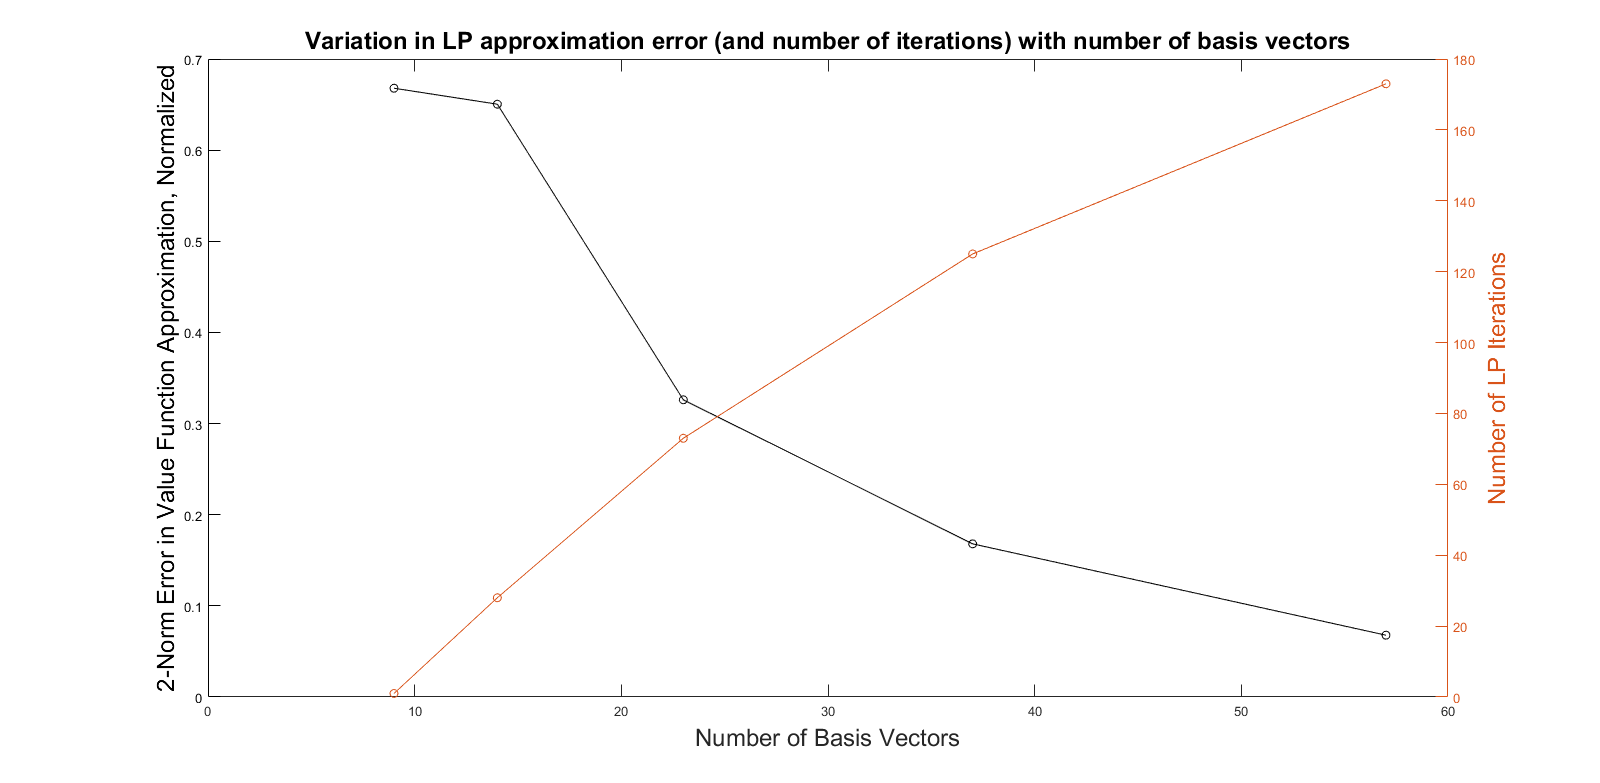
\includegraphics[scale=0.25]{ApproxErr_vs_NumIter.png}}
\caption{Variation in approximation error and solution time with number of basis vectors added. Test size: N=$6\cdot5=30$, M=10.}
\label{fig:ApproxVsIter}This shows that the approximation error can indeed be made arbitarily small by adding more basis vectors.
\end{figure} %Additionally, Figure  also shows the approximation error decreasing for a medium-sized problem as more basis vectors are added. 


%Finally, in addition to quantifying the error for LP, the LP is also compared to DP based on computational complexity. Table II provides simulation results for the number of iterations as the model size and tolerances (of \textit{both} programs) are varied.

%The experimental results in this table show that LP generally takes longer to converge for small problems, but is faster for large problems. Hence, this suggests that the LP formulation may be a more efficient program for this two-storage application.

%While the size of problems and number of cost evaluations were compared in Sections 4 and 6 for the general case, the number of iterations very application-dependent, as previously explained.

\section{Conclusion}
In conclusion, this paper has developed and optimized a model for energy transfers from two parallel storage devices satisfy a random demand. The model is an extension of the case with a single storage device, and was formulated using dynamic programming. Its optimal control policy can be applied to exactly satisfy a real-time demand, making it suitable for applications such as EVs.

Based on the timescales associated with this application, the DP was formulated as an infinite horizon problem. Most importantly, in order to resolve the curse of dimensionality, the solution was approximated by solving an approximate LP. To this end, the basis functions for the linear approximation were generated through a combination of state aggregation and monomials of state indices.

Lastly, the final program was simulated with three classes of demand to determine the optimal control in each case. As expected, it was found that high-energy or steady demands lead to more use of the battery, whereas fluctuating demand leads to more use of the complementary storage device. This means the policy produced by the program should work to reduce battery degradation, based on literature reviewed.

The final simulation results confirm that the approximate LP does allow for determining an optimal policy. Further work remains to be done to incorporate regenerative braking into this model.

\printbibliography

\end{document}